% begin module newtons-method-def
\begin{frame}
Goal: find a root $r$ of $f(x)$.
\begin{columns}[c]
\column{.45\textwidth}
\ \only<handout:0| -2>{%
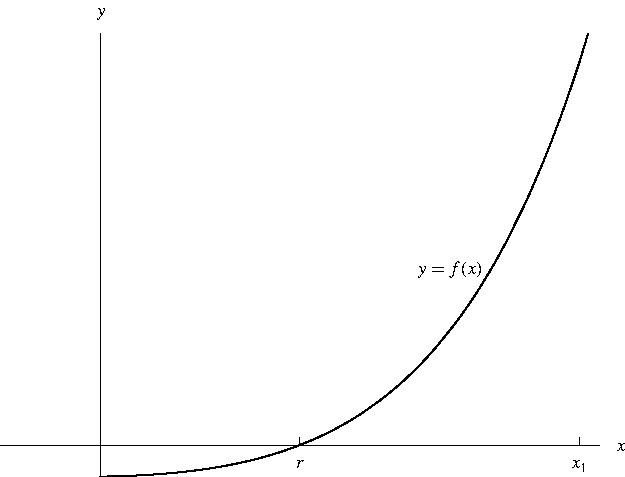
\includegraphics[height=4cm]{newtons-method/pictures/04-08-newtona.pdf}%
}%
\only<handout:0| 3-5,10-16>{%
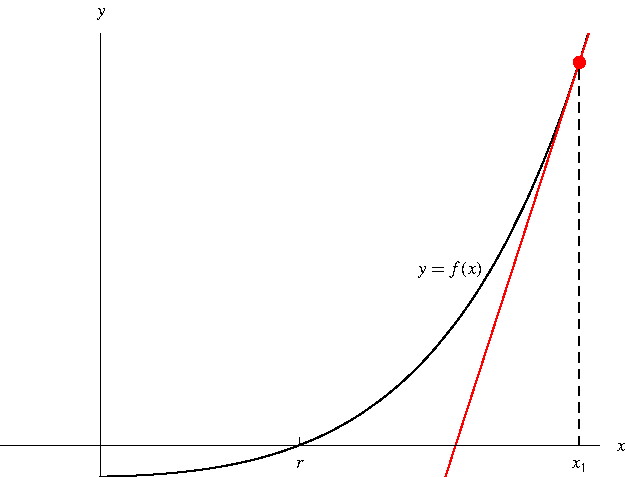
\includegraphics[height=4cm]{newtons-method/pictures/04-08-newtonb.pdf}%
}%
\only<handout:0| 6-7,17-22>{%
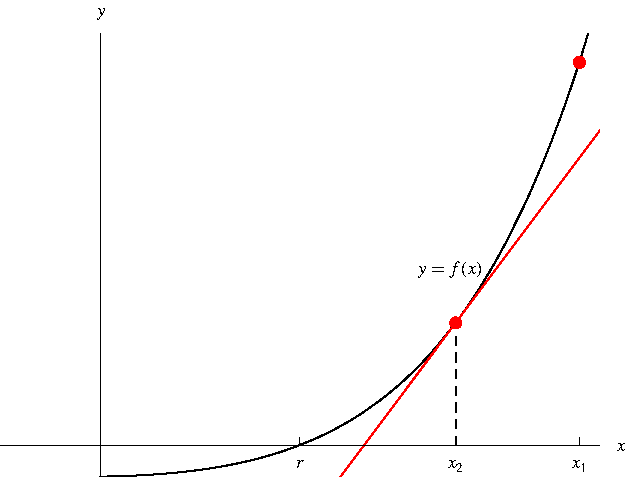
\includegraphics[height=4cm]{newtons-method/pictures/04-08-newtonc.pdf}%
}%
\only<handout:0| 8>{%
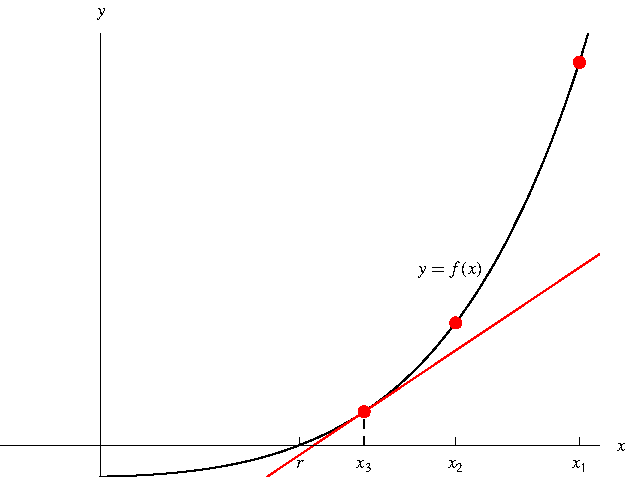
\includegraphics[height=4cm]{newtons-method/pictures/04-08-newtond.pdf}%
}%
\only<9,23->{%
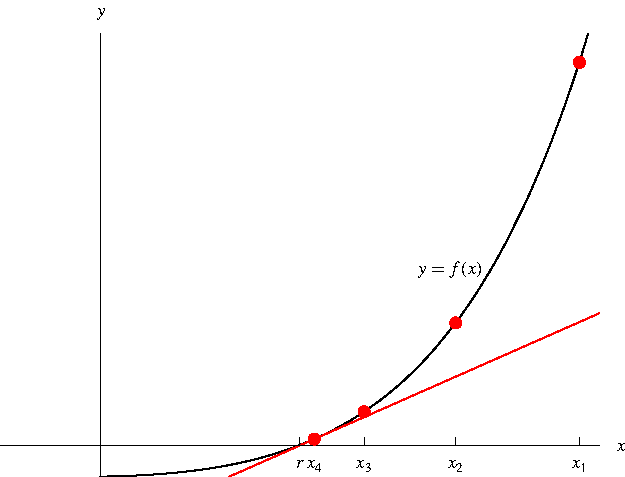
\includegraphics[height=4cm]{newtons-method/pictures/04-08-newtone.pdf}%
}%

\column{.55\textwidth}

\begin{itemize}
\item<2->  Pick a number $x_1$.
\item<3-| alert@10-12>  Find the tangent to $f$ at $(x_1, f(x_1))$.
\item<4-| alert@13-15>  Call the $x$-intercept of this line $x_2$.
\item<5->  Repeat the process using $x_2$ in the place of $x_1$:
\item<6-| alert@17-19>  Find the tangent to $f$ at $(x_2, f(x_2))$.
\item<7-| alert@20-22>  Call the $x$-intercept of this line $x_3$.
\end{itemize}
\end{columns}

\begin{columns}[c]
\column{.55\textwidth}
\abovedisplayskip=0pt
\belowdisplayskip=-15pt
\begin{align*}
\uncover<10-15,17-22>{\text{Equation:}}\quad
\uncover<10-15,17-22>{y - \uncover<12-15,19-22>{\alert<handout:0| 12,19>{f(x_{\only<handout:0| -15>{1}\only<handout:0| 16->{2}})}}} & \uncover<10-15,17-22>{=}  \uncover<11-15,18-22>{\alert<handout:0| 11,18>{f'(x_{\only<handout:0| -15>{1}\only<handout:0| 16->{2}})}}\uncover<10-15,17-22>{(x-\uncover<12-15,19-22>{\alert<handout:0| 12,19>{x_{\only<handout:0| -15>{1}\only<handout:0| 16->{2}}}})}\\
\uncover<13-15,20-22>{\text{$x$-intercept:}}\quad
\uncover<13-15,20-22>{\alert<handout:0| 13,20>{0} - f(x_{\only<handout:0| -15>{1}\only<handout:0| 16->{2}})} & \uncover<13-15,20-22>{=}  \uncover<13-15,20-22>{f'(x_{\only<handout:0| -15>{1}\only<handout:0| 16->{2}})(\alert<handout:0| 13,20>{x_{\only<handout:0| -15>{2}\only<handout:0| 16->{3}}}-x_{\only<handout:0| -15>{1}\only<handout:0| 16->{2}})}\\
\uncover<14-15,21-22>{f'(x_{\only<handout:0| -15>{1}\only<handout:0| 16->{2}})x_{\only<handout:0| -15>{1}\only<handout:0| 16->{2}} - f(x_{\only<handout:0| -15>{1}\only<handout:0| 16->{2}})} & \uncover<14-15,21-22>{=}  \uncover<14-15,21-22>{f'(x_{\only<handout:0| -15>{1}\only<handout:0| 16->{2}})x_{\only<handout:0| -15>{2}\only<handout:0| 16->{3}}}\\
\uncover<15,22>{x_{\only<handout:0| -15>{2}\only<handout:0| 16->{3}}} & \uncover<15,22>{=}  \uncover<15,22>{x_{\only<handout:0| -15>{1}\only<handout:0| 16->{2}} - \frac{f(x_{\only<handout:0| -15>{1}\only<handout:0| 16->{2}})}{f'(x_{\only<handout:0| -15>{1}\only<handout:0| 16->{2}})}}
\end{align*}
\column{.45\textwidth}
\[
\uncover<16->{%
x_2 = x_1 - \frac{f(x_1)}{f'(x_1)}%
}%
\]
\[
\uncover<23->{%
x_3 = x_2 - \frac{f(x_2)}{f'(x_2)}%
}%
\]
\[
\uncover<24->{%
x_{n+1} = x_n - \frac{f(x_n)}{f'(x_n)}%
}%
\]
\end{columns}
\end{frame}
% end module newtons-method-def
